\documentclass[11pt]{article}\usepackage[]{graphicx}\usepackage[dvipsnames]{xcolor}
% maxwidth is the original width if it is less than linewidth
% otherwise use linewidth (to make sure the graphics do not exceed the margin)
\makeatletter
\def\maxwidth{ %
  \ifdim\Gin@nat@width>\linewidth
    \linewidth
  \else
    \Gin@nat@width
  \fi
}
\makeatother

\definecolor{fgcolor}{rgb}{0.345, 0.345, 0.345}
\newcommand{\hlnum}[1]{\textcolor[rgb]{0.686,0.059,0.569}{#1}}%
\newcommand{\hlsng}[1]{\textcolor[rgb]{0.192,0.494,0.8}{#1}}%
\newcommand{\hlcom}[1]{\textcolor[rgb]{0.678,0.584,0.686}{\textit{#1}}}%
\newcommand{\hlopt}[1]{\textcolor[rgb]{0,0,0}{#1}}%
\newcommand{\hldef}[1]{\textcolor[rgb]{0.345,0.345,0.345}{#1}}%
\newcommand{\hlkwa}[1]{\textcolor[rgb]{0.161,0.373,0.58}{\textbf{#1}}}%
\newcommand{\hlkwb}[1]{\textcolor[rgb]{0.69,0.353,0.396}{#1}}%
\newcommand{\hlkwc}[1]{\textcolor[rgb]{0.333,0.667,0.333}{#1}}%
\newcommand{\hlkwd}[1]{\textcolor[rgb]{0.737,0.353,0.396}{\textbf{#1}}}%
\let\hlipl\hlkwb

\usepackage{framed}
\makeatletter
\newenvironment{kframe}{%
 \def\at@end@of@kframe{}%
 \ifinner\ifhmode%
  \def\at@end@of@kframe{\end{minipage}}%
  \begin{minipage}{\columnwidth}%
 \fi\fi%
 \def\FrameCommand##1{\hskip\@totalleftmargin \hskip-\fboxsep
 \colorbox{shadecolor}{##1}\hskip-\fboxsep
     % There is no \\@totalrightmargin, so:
     \hskip-\linewidth \hskip-\@totalleftmargin \hskip\columnwidth}%
 \MakeFramed {\advance\hsize-\width
   \@totalleftmargin\z@ \linewidth\hsize
   \@setminipage}}%
 {\par\unskip\endMakeFramed%
 \at@end@of@kframe}
\makeatother

\definecolor{shadecolor}{rgb}{.97, .97, .97}
\definecolor{messagecolor}{rgb}{0, 0, 0}
\definecolor{warningcolor}{rgb}{1, 0, 1}
\definecolor{errorcolor}{rgb}{1, 0, 0}
\newenvironment{knitrout}{}{} % an empty environment to be redefined in TeX

\usepackage{alltt}
\usepackage[utf8]{inputenc}
\usepackage[T1]{fontenc}
\usepackage{lmodern}
\usepackage{amsmath, amssymb, amsthm, graphicx, physics}
\usepackage{enumitem}
\usepackage{geometry}
\usepackage[dvipsnames]{xcolor}
\definecolor{EvanPink}{rgb}{0.85, 0.13, 0.55}
\usepackage[colorlinks=true,
            linkcolor=OliveGreen,
            urlcolor=EvanPink,
            citecolor=OliveGreen]{hyperref}
\usepackage{cleveref}
\usepackage{etoolbox}
\newenvironment{solution}{%
  \par\noindent\textit{Solution.}\ }{\qed}
\newtheoremstyle{problemstyle}
  {1em}   
  {1em}   
  {}      
  {}      
  {\bfseries} 
  {.}     
  {0.5em} 
  {}      
\theoremstyle{problemstyle}
\newtheorem{problem}{Problem}[section]
\crefname{problem}{Problem}{Problems}
\Crefname{problem}{Problem}{Problems}
\def\bN{\mathbb{N}}
\def\bR{\mathbb{R}}
\def\bZ{\mathbb{Z}}
\def\bQ{\mathbb{Q}}
\def\mM{\mathcal{M}}
\def\mR{\mathcal{R}}
\def\mN{\mathcal{N}}
\def\mE{\mathcal{E}}
\def\mA{\mathcal{A}}
%%%%%%%%%%%%%%%Setting Page Sizes %%%%%%%%%%%%
\setlength{\parindent}{0in}
\setlength{\parskip}{\baselineskip}
\setlength{\textheight}{9in}
\setlength{\textwidth}{6.3in}
\setlength{\topmargin}{-0.6in}
\setlength{\evensidemargin}{-.5in}
\setlength{\oddsidemargin}{0in}
%%%%%%%%%%%%%%%%%%%%%%%%%%%%%%%%%%%%%%%%%%%

%%%%%%%%%%%%To make R commands appear in different Color%%%%%%%%%%
\usepackage{color}
\usepackage{fancyvrb} % Verbatim
%\usepackage{Sweave} % for R code
\usepackage{color}
\definecolor{codecolor}{RGB}{114,12,112}
\DefineVerbatimEnvironment{Sinput}{Verbatim}{formatcom=\color{codecolor}}
\DefineVerbatimEnvironment{Soutput}{Verbatim}{formatcom=\color{codecolor}}
\DefineVerbatimEnvironment{Scode}{Verbatim}{formatcom=\color{codecolor}}
\DefineVerbatimEnvironment{Sin}{Verbatim}{formatcom=\color{codecolor}}
\DefineVerbatimEnvironment{Sout}{Verbatim}{formatcom=\color{codecolor}}
%%%%%%%%%%%%%%%%%%%%%%%%%%%%%%%%%%%%%%%%%%%%%%%%%%%%%%%%%%%%%%%%

\IfFileExists{upquote.sty}{\usepackage{upquote}}{}
\begin{document}

{\bf Arkaraj Mukherjee: }
{\bf Homework 4}
\\
\begin{knitrout}
\definecolor{shadecolor}{rgb}{0.969, 0.969, 0.969}\color{fgcolor}\begin{kframe}
\begin{alltt}
\hlkwd{library}\hldef{(}\hlsng{"tidyverse"}\hldef{);}
\hlkwd{setwd}\hldef{(}\hlsng{"~/isi_bmath/sem_II/intro_to_statistics_and_computation_with_data"}\hldef{);}
\end{alltt}
\end{kframe}
\end{knitrout}

\begin{enumerate}[label=\arabic*.]
    \item
    \begin{enumerate}[label=(\alph*)]
\item We assume that the pdf for a \texttt{geom}($p$) and \texttt{negativebinomial}($r,p$) are $p_{\texttt{geom}}(k)=p(1-p)^{k-1}$ for and $p_{\texttt{negativebinomial}}(k)=\binom{k-1}{r-1}p^r(1-p)^{k-r}$ for $k=1,2,\ldots$
\begin{knitrout}
\definecolor{shadecolor}{rgb}{0.969, 0.969, 0.969}\color{fgcolor}\begin{kframe}
\begin{alltt}
\hldef{p} \hlkwb{=} \hlnum{0.3}
\hlkwd{set.seed}\hldef{(}\hlnum{82407}\hldef{)}
\hldef{geom} \hlkwb{=} \hlkwd{vector}\hldef{(}\hlsng{"numeric"}\hldef{,} \hlkwc{length} \hldef{=} \hlnum{100}\hldef{)}
\hlkwa{for}\hldef{(i} \hlkwa{in} \hlnum{1}\hlopt{:}\hlnum{100}\hldef{) \{}
    \hldef{B} \hlkwb{=} \hlnum{0}
    \hlkwa{while}\hldef{(B} \hlopt{==} \hlnum{0}\hldef{) \{}
        \hldef{U} \hlkwb{=} \hlkwd{runif}\hldef{(}\hlnum{1}\hldef{,} \hlkwc{min} \hldef{=} \hlnum{0}\hldef{,} \hlkwc{max} \hldef{=} \hlnum{1}\hldef{)}
        \hldef{B} \hlkwb{=} \hlkwd{as.numeric}\hldef{(U}\hlopt{<}\hldef{p)}
        \hldef{geom[i]} \hlkwb{=} \hldef{geom[i]} \hlopt{+} \hlnum{1}
    \hldef{\}}
\hldef{\}}
\hlkwd{head}\hldef{(geom,} \hlkwc{n} \hldef{=} \hlnum{10}\hldef{)}
\end{alltt}
\begin{verbatim}
##  [1]  3  1  3 15  5  2  1  1  2  4
\end{verbatim}
\begin{alltt}
\hldef{p} \hlkwb{=} \hlnum{0.7}
\hldef{r} \hlkwb{=} \hlnum{4}
    \hldef{nb} \hlkwb{=} \hlkwd{vector}\hldef{(}\hlsng{"numeric"}\hldef{,} \hlkwc{length} \hldef{=} \hlnum{100}\hldef{)}
    \hlkwa{for}\hldef{(i} \hlkwa{in} \hlnum{1}\hlopt{:}\hlnum{100}\hldef{) \{}
        \hldef{B} \hlkwb{=} \hlnum{0}
        \hlkwa{while}\hldef{(B} \hlopt{<} \hldef{r) \{}
            \hldef{U} \hlkwb{=} \hlkwd{runif}\hldef{(}\hlnum{1}\hldef{,} \hlkwc{min} \hldef{=} \hlnum{0}\hldef{,} \hlkwc{max} \hldef{=} \hlnum{1}\hldef{)}
            \hldef{B} \hlkwb{=} \hldef{B} \hlopt{+} \hlkwd{as.numeric}\hldef{(U}\hlopt{<}\hldef{p)}
            \hldef{nb[i]} \hlkwb{=} \hldef{nb[i]} \hlopt{+} \hlnum{1}
        \hldef{\}}
    \hldef{\}}
    \hlkwd{head}\hldef{(nb,} \hlkwc{n} \hldef{=} \hlnum{10}\hldef{)}
\end{alltt}
\begin{verbatim}
##  [1] 4 7 5 7 4 7 5 6 7 4
\end{verbatim}
\end{kframe}
\end{knitrout}
    
    \item We assume that the pdf for cauchy distribution is $p_{\texttt{cauchy}}(x)=\pi^{-1}(1+x^2)^{-1}$ and use the inverse CDF method discussed in class
\begin{knitrout}
\definecolor{shadecolor}{rgb}{0.969, 0.969, 0.969}\color{fgcolor}\begin{kframe}
\begin{alltt}
\hldef{cau} \hlkwb{=} \hlkwd{tan}\hldef{(pi} \hlopt{*} \hldef{(}\hlkwd{runif}\hldef{(}\hlnum{100}\hldef{)}\hlopt{-}\hlnum{1}\hlopt{/}\hlnum{2}\hldef{));}
\hlkwd{round}\hldef{(}\hlkwd{head}\hldef{(cau,} \hlkwc{n} \hldef{=} \hlnum{5}\hldef{),} \hlkwc{digits} \hldef{=} \hlnum{3}\hldef{)}
\end{alltt}
\begin{verbatim}
## [1] -1.989  0.731 -2.006 -1.350 -0.106
\end{verbatim}
\end{kframe}
\end{knitrout}
    \end{enumerate}
    \item
\begin{knitrout}
\definecolor{shadecolor}{rgb}{0.969, 0.969, 0.969}\color{fgcolor}\begin{kframe}
\begin{alltt}
\hldef{U} \hlkwb{=} \hlkwd{runif}\hldef{(}\hlnum{100}\hldef{,}\hlkwc{max}\hldef{=}\hlnum{1}\hldef{,}\hlkwc{min}\hldef{=}\hlnum{0}\hldef{)}
\hldef{E} \hlkwb{=} \hlkwd{rexp}\hldef{(}\hlnum{100}\hldef{,}\hlkwc{rate}\hldef{=}\hlnum{1}\hldef{)}
\hlkwd{qqnorm}\hldef{(U)}
\hlkwd{qqline}\hldef{(U)}
\end{alltt}
\end{kframe}
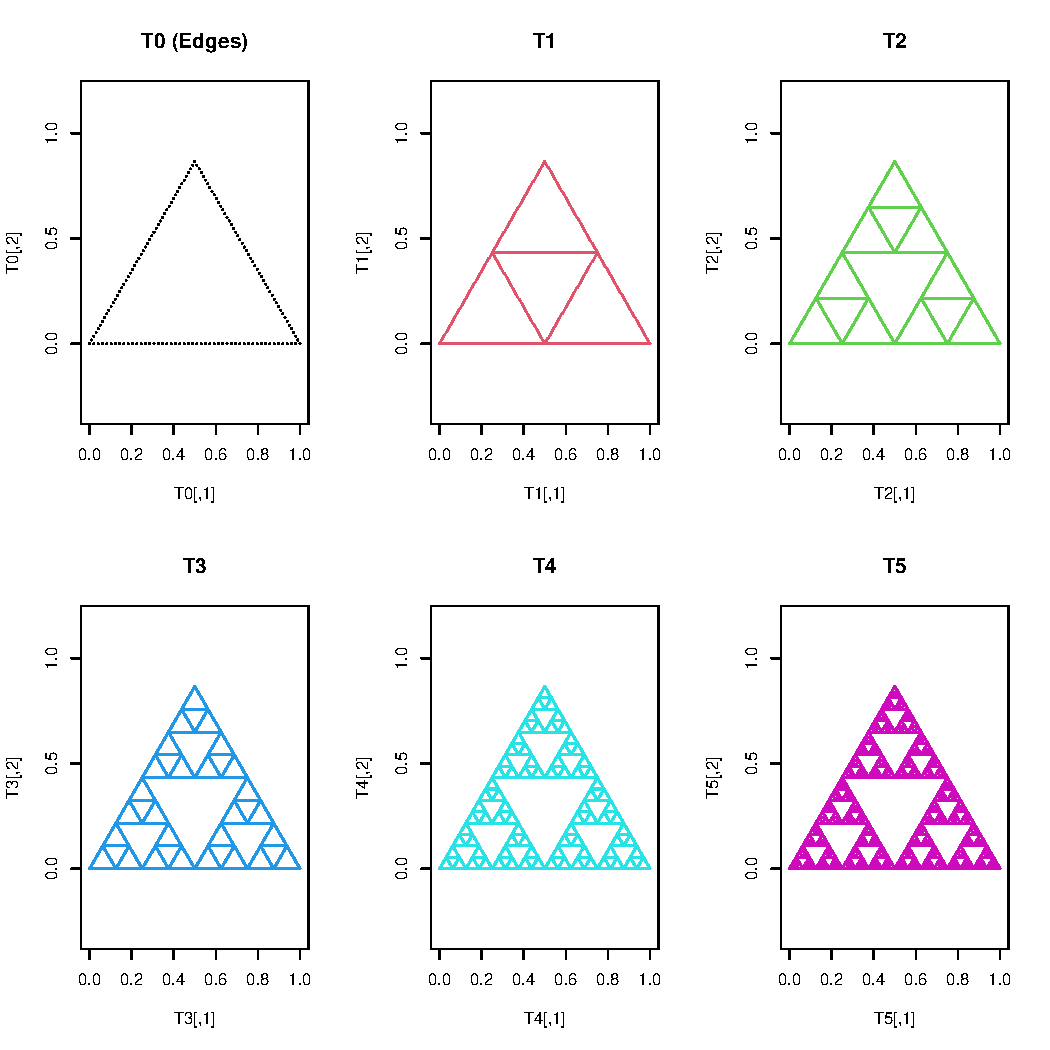
\includegraphics[width=\maxwidth]{figure/unnamed-chunk-4-1} 
\begin{kframe}\begin{alltt}
\hlkwd{qqnorm}\hldef{(E)}
\hlkwd{qqline}\hldef{(E)}
\end{alltt}
\end{kframe}
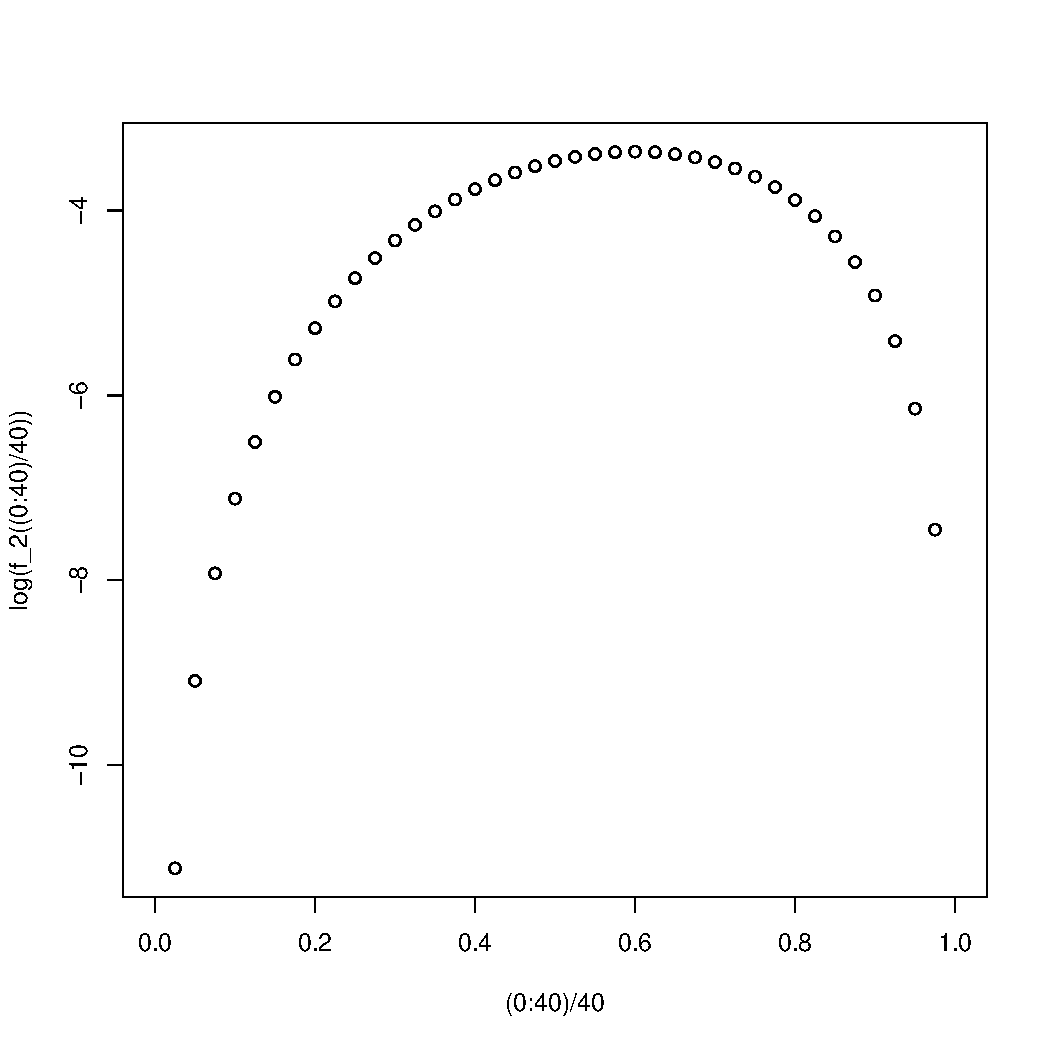
\includegraphics[width=\maxwidth]{figure/unnamed-chunk-4-2} 
\end{knitrout}
        These plots show that neither sample is normally distributed because the points do not follow the straight diagonal line. The Exponential plot curves upwards, showing the data is skewed instead of symmetrical. The Uniform plot forms an 'S' shape, showing that the data is cut off at the ends ($0$ and $1$) rather than spreading out widely like a normal distribution.
    \item \begin{enumerate}[label=(\alph*)]
        \item[(0)] If $X$ is a binomial random variable with parameters $N,p$ then,
        $$\mathbb{E}[X]=Np\text{ and, }\mathbb{E}[X^2]=Np(1-p)+N^2p^2$$
        \texttt{phat} and \texttt{Nhat} are approximations of $p$ and $N$ respectively which we get from solving for $N,p$ using the mean of our data and the square mean, its an approximation as our means may be close to the theoretical means but they needn't be equal to the theoretical mean.
        \item 
\begin{knitrout}
\definecolor{shadecolor}{rgb}{0.969, 0.969, 0.969}\color{fgcolor}\begin{kframe}
\begin{alltt}
\hldef{n} \hlkwb{=} \hlnum{100}
\hldef{N} \hlkwb{=} \hlnum{20}
\hldef{p} \hlkwb{=} \hlnum{0.4}
\hldef{x} \hlkwb{=} \hlkwd{rbinom}\hldef{(n,N,p)}
\hldef{m1} \hlkwb{=} \hlkwd{mean}\hldef{(x)}
\hldef{m2} \hlkwb{=} \hlkwd{mean}\hldef{(x}\hlopt{^}\hlnum{2}\hldef{)}
\hldef{Nhat} \hlkwb{=} \hldef{m1}\hlopt{^}\hlnum{2} \hlopt{/} \hldef{(m1} \hlopt{-} \hldef{(m2} \hlopt{-} \hldef{m1}\hlopt{^}\hlnum{2}\hldef{))}
\hldef{phat} \hlkwb{=} \hldef{(m1} \hlopt{-} \hldef{(m2} \hlopt{-} \hldef{m1}\hlopt{^}\hlnum{2}\hldef{))} \hlopt{/} \hldef{m1}
\hldef{Nhat} \hlopt{-} \hldef{N}
\end{alltt}
\begin{verbatim}
## [1] 8.183946
\end{verbatim}
\begin{alltt}
\hldef{phat} \hlopt{-} \hldef{p}
\end{alltt}
\begin{verbatim}
## [1] -0.1179245
\end{verbatim}
\end{kframe}
\end{knitrout}
        \item 
\begin{knitrout}
\definecolor{shadecolor}{rgb}{0.969, 0.969, 0.969}\color{fgcolor}\begin{kframe}
\begin{alltt}
\hldef{n} \hlkwb{=} \hlnum{1000}
\hldef{N} \hlkwb{=} \hlnum{20}
\hldef{p} \hlkwb{=} \hlnum{0.4}
\hldef{x} \hlkwb{=} \hlkwd{rbinom}\hldef{(n,N,p)}
\hldef{m1} \hlkwb{=} \hlkwd{mean}\hldef{(x)}
\hldef{m2} \hlkwb{=} \hlkwd{mean}\hldef{(x}\hlopt{^}\hlnum{2}\hldef{)}
\hldef{Nhat} \hlkwb{=} \hldef{m1}\hlopt{^}\hlnum{2} \hlopt{/} \hldef{(m1} \hlopt{-} \hldef{(m2} \hlopt{-} \hldef{m1}\hlopt{^}\hlnum{2}\hldef{))}
\hldef{phat} \hlkwb{=} \hldef{(m1} \hlopt{-} \hldef{(m2} \hlopt{-} \hldef{m1}\hlopt{^}\hlnum{2}\hldef{))} \hlopt{/} \hldef{m1}
\hldef{Nhat} \hlopt{-} \hldef{N}
\end{alltt}
\begin{verbatim}
## [1] 2.006175
\end{verbatim}
\begin{alltt}
\hldef{phat} \hlopt{-} \hldef{p}
\end{alltt}
\begin{verbatim}
## [1] -0.04010101
\end{verbatim}
\end{kframe}
\end{knitrout}
        It does change, the error is much smaller now.
        \item 
\begin{knitrout}
\definecolor{shadecolor}{rgb}{0.969, 0.969, 0.969}\color{fgcolor}\begin{kframe}
\begin{alltt}
\hldef{n} \hlkwb{=} \hlnum{100}\hldef{;}
\hldef{N} \hlkwb{=} \hlnum{10}\hldef{;}
\hldef{p} \hlkwb{=} \hlnum{0.9}\hldef{;}
\hldef{x} \hlkwb{=} \hlkwd{rbinom}\hldef{(n,N,p);}
\hldef{m1} \hlkwb{=} \hlkwd{mean}\hldef{(x);}
\hldef{m2} \hlkwb{=} \hlkwd{mean}\hldef{(x}\hlopt{^}\hlnum{2}\hldef{);}
\hldef{Nhat} \hlkwb{=} \hldef{m1}\hlopt{^}\hlnum{2} \hlopt{/} \hldef{(m1} \hlopt{-} \hldef{(m2} \hlopt{-} \hldef{m1}\hlopt{^}\hlnum{2}\hldef{));}
\hldef{phat} \hlkwb{=} \hldef{(m1} \hlopt{-} \hldef{(m2} \hlopt{-} \hldef{m1}\hlopt{^}\hlnum{2}\hldef{))} \hlopt{/} \hldef{m1;}
\hldef{Nhat} \hlopt{-} \hldef{N}
\end{alltt}
\begin{verbatim}
## [1] -0.2004711
\end{verbatim}
\begin{alltt}
\hldef{phat} \hlopt{-} \hldef{p}
\end{alltt}
\begin{verbatim}
## [1] 0.02147287
\end{verbatim}
\begin{alltt}
\hldef{n} \hlkwb{=} \hlnum{1000}\hldef{;}
\hldef{N} \hlkwb{=} \hlnum{10}\hldef{;}
\hldef{p} \hlkwb{=} \hlnum{0.9}\hldef{;}
\hldef{x} \hlkwb{=} \hlkwd{rbinom}\hldef{(n,N,p);}
\hldef{m1} \hlkwb{=} \hlkwd{mean}\hldef{(x);}
\hldef{m2} \hlkwb{=} \hlkwd{mean}\hldef{(x}\hlopt{^}\hlnum{2}\hldef{);}
\hldef{Nhat} \hlkwb{=} \hldef{m1}\hlopt{^}\hlnum{2} \hlopt{/} \hldef{(m1} \hlopt{-} \hldef{(m2} \hlopt{-} \hldef{m1}\hlopt{^}\hlnum{2}\hldef{));}
\hldef{phat} \hlkwb{=} \hldef{(m1} \hlopt{-} \hldef{(m2} \hlopt{-} \hldef{m1}\hlopt{^}\hlnum{2}\hldef{))} \hlopt{/} \hldef{m1;}
\hldef{Nhat} \hlopt{-} \hldef{N}
\end{alltt}
\begin{verbatim}
## [1] 0.005119977
\end{verbatim}
\begin{alltt}
\hldef{phat} \hlopt{-} \hldef{p}
\end{alltt}
\begin{verbatim}
## [1] -0.002759385
\end{verbatim}
\end{kframe}
\end{knitrout}
    \end{enumerate}
    \item \begin{enumerate}[label=(\alph*)]
        \item 
\begin{knitrout}
\definecolor{shadecolor}{rgb}{0.969, 0.969, 0.969}\color{fgcolor}\begin{kframe}
\begin{alltt}
\hldef{x} \hlkwb{=} \hlkwd{seq}\hldef{(}\hlopt{-}\hlnum{2}\hldef{,} \hlnum{2}\hldef{,} \hlkwc{by} \hldef{=} \hlnum{0.1}\hldef{)}
\hlkwd{plot}\hldef{(x,}\hlkwd{pnorm}\hldef{(x,} \hlkwc{mean} \hldef{=} \hlnum{0}\hldef{,} \hlkwc{sd} \hldef{=} \hlnum{1}\hldef{))}
\end{alltt}
\end{kframe}
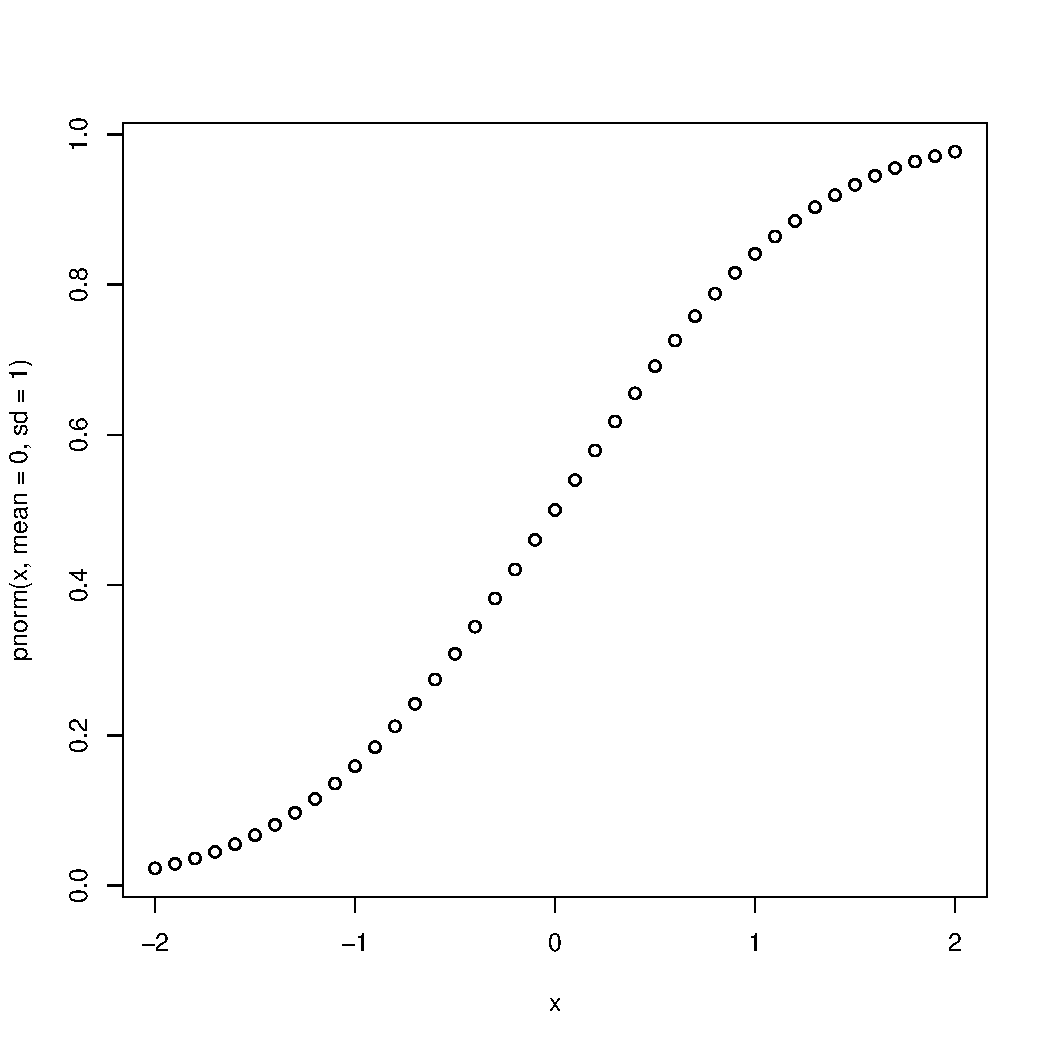
\includegraphics[width=\maxwidth]{figure/unnamed-chunk-8-1} 
\end{knitrout}
        \item We use the fact that $P(Z\leq x)=P(Y\leq x\cdot\sqrt{mp(1-p)}+mp)$
\begin{knitrout}
\definecolor{shadecolor}{rgb}{0.969, 0.969, 0.969}\color{fgcolor}\begin{kframe}
\begin{alltt}
\hldef{m} \hlkwb{=} \hlnum{100}
\hldef{p} \hlkwb{=} \hlnum{0.4}
\hldef{ev} \hlkwb{=} \hldef{m}\hlopt{*}\hldef{p}
\hldef{sd} \hlkwb{=} \hlkwd{sqrt}\hldef{(m}\hlopt{*}\hldef{p}\hlopt{*}\hldef{(}\hlnum{1}\hlopt{-}\hldef{p))}
\hlkwd{plot}\hldef{(x,}\hlkwd{pbinom}\hldef{(sd}\hlopt{*}\hldef{x}\hlopt{+}\hldef{ev,} \hlkwc{size} \hldef{= m,} \hlkwc{prob} \hldef{= p))}
\end{alltt}
\end{kframe}
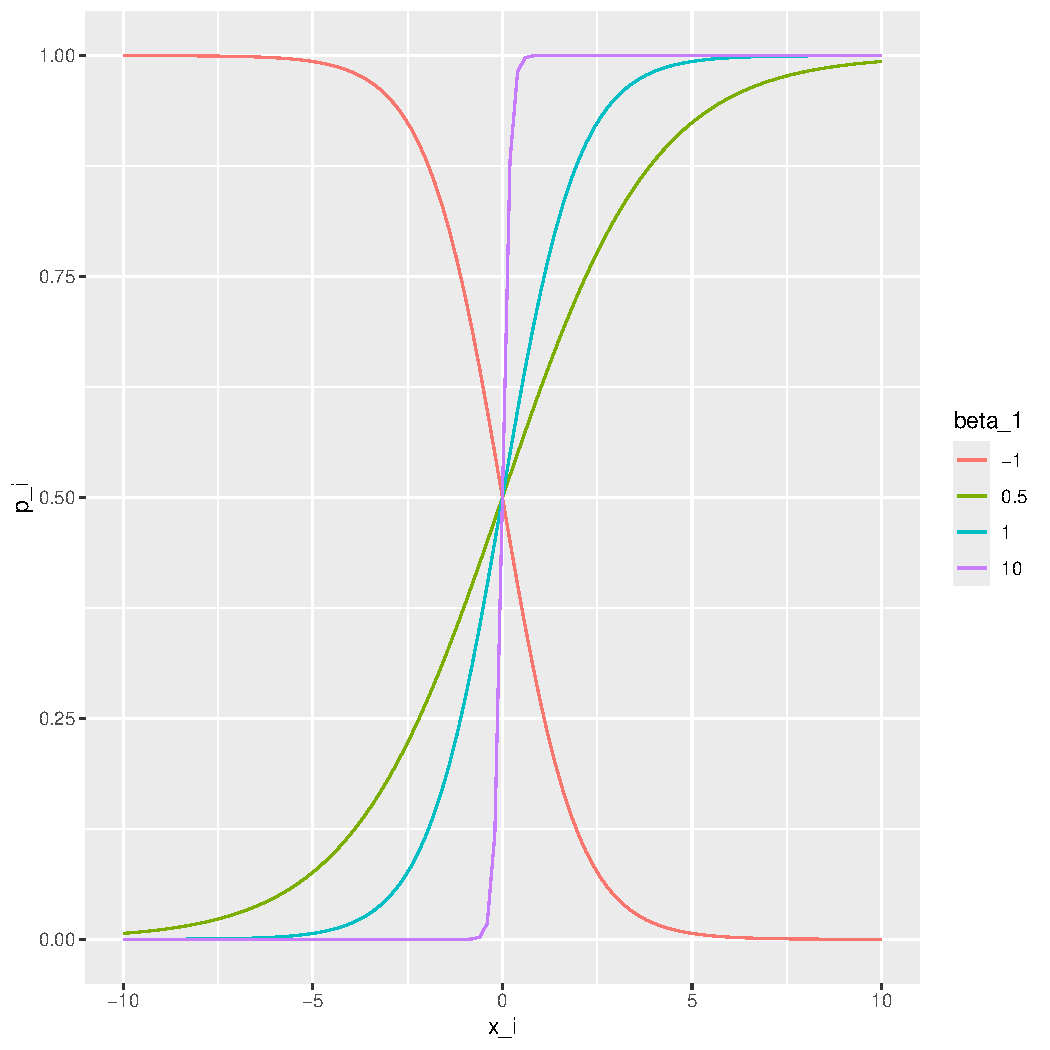
\includegraphics[width=\maxwidth]{figure/unnamed-chunk-9-1} 
\end{knitrout}
        \item 
\begin{knitrout}
\definecolor{shadecolor}{rgb}{0.969, 0.969, 0.969}\color{fgcolor}\begin{kframe}
\begin{alltt}
\hldef{m} \hlkwb{<-} \hlnum{100}
\hldef{p} \hlkwb{<-} \hlnum{0.4}
\hldef{binom_samples} \hlkwb{<-} \hlkwd{rbinom}\hldef{(}\hlnum{1000}\hldef{,} \hlkwc{size} \hldef{= m,} \hlkwc{prob} \hldef{= p)}
\hldef{mu_val} \hlkwb{<-} \hldef{m} \hlopt{*} \hldef{p}
\hldef{sigma_val} \hlkwb{<-} \hlkwd{sqrt}\hldef{(m} \hlopt{*} \hldef{p} \hlopt{*} \hldef{(}\hlnum{1} \hlopt{-} \hldef{p))}
\hldef{df} \hlkwb{<-} \hlkwd{data.frame}\hldef{(}\hlkwc{vals} \hldef{= binom_samples)}
\hlkwd{ggplot}\hldef{(df,} \hlkwd{aes}\hldef{(}\hlkwc{x} \hldef{= vals))} \hlopt{+}
\hlkwd{geom_histogram}\hldef{(}\hlkwd{aes}\hldef{(}\hlkwc{y} \hldef{= ..density..),} \hlkwc{binwidth} \hldef{=} \hlnum{1}\hldef{)} \hlopt{+}
\hlkwd{stat_function}\hldef{(}\hlkwc{fun} \hldef{= dnorm,} \hlkwc{args} \hldef{=} \hlkwd{list}\hldef{(}\hlkwc{mean} \hldef{= mu_val,} \hlkwc{sd} \hldef{= sigma_val))}
\end{alltt}
\end{kframe}
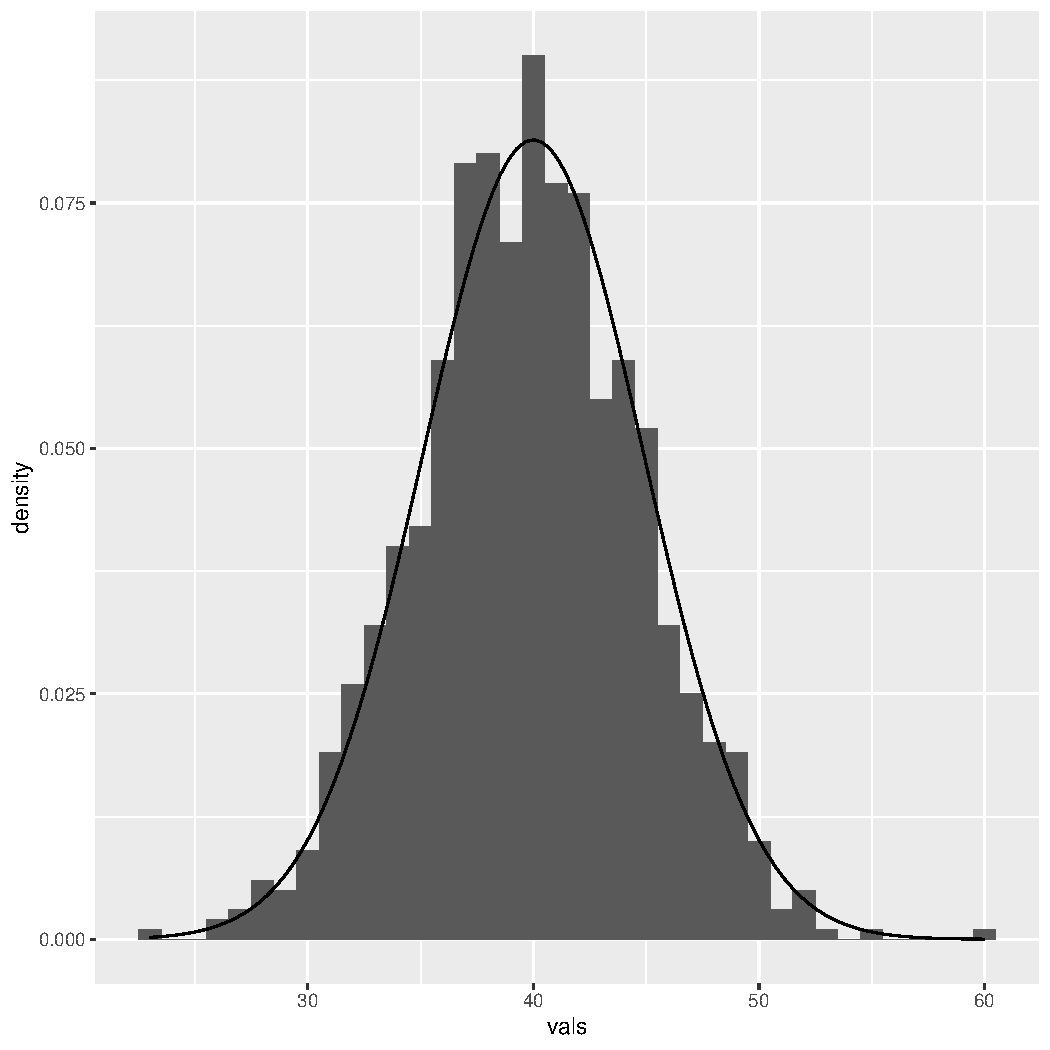
\includegraphics[width=\maxwidth]{figure/unnamed-chunk-10-1} 
\end{knitrout}
    \end{enumerate}
    \item 
\begin{knitrout}
\definecolor{shadecolor}{rgb}{0.969, 0.969, 0.969}\color{fgcolor}\begin{kframe}
\begin{alltt}
\hldef{x} \hlkwb{=} \hlkwd{c}\hldef{(}\hlnum{1}\hldef{,}\hlnum{2}\hldef{,}\hlnum{3}\hldef{,}\hlnum{4}\hldef{,}\hlnum{5}\hldef{,}\hlnum{6}\hldef{)}
\hlcom{#this creates a vector with the entries above to serve as the possible samples}
\hldef{probx} \hlkwb{=} \hlkwd{c}\hldef{(}\hlnum{1}\hlopt{/}\hlnum{6}\hldef{,}\hlnum{1}\hlopt{/}\hlnum{6}\hldef{,}\hlnum{1}\hlopt{/}\hlnum{6}\hldef{,}\hlnum{1}\hlopt{/}\hlnum{6}\hldef{,}\hlnum{1}\hlopt{/}\hlnum{6}\hldef{,}\hlnum{1}\hlopt{/}\hlnum{6}\hldef{)}
\hlcom{#this creates another vector but this serves as the probability of }
\hlcom{#getting some sample}
\hldef{Rolls} \hlkwb{=} \hlkwd{sample}\hldef{(x,} \hlkwc{size} \hldef{=} \hlnum{1500}\hldef{,} \hlkwc{replace} \hldef{= T,} \hlkwc{prob} \hldef{= probx)}
\hlcom{#this samples from the distribution described by x and probx 1500 }
\hlcom{#times with replacement and stores these in Rolls}
\hldef{Rollm} \hlkwb{=} \hlkwd{matrix}\hldef{(Rolls,} \hlkwc{nrow} \hldef{=} \hlnum{5}\hldef{)}
\hlcom{#This creates a matrix out of Rolls by wrapping the vector such that }
\hlcom{#the matrix has 5 rows, it will have 1500/5=300 columns}
\hldef{Rollsums} \hlkwb{=} \hlkwd{apply}\hldef{(Rollm,} \hlnum{2}\hldef{, sum)}
\hlcom{#This sums the entries in each column and puts them in Rollsums, if we}
\hlcom{#had 1 instead of 2 there then it'd have summed the rows}
\hlkwd{library}\hldef{(ggplot2)}
\hlcom{#self explanatory}
\hldef{density} \hlkwb{=} \hlkwa{function}\hldef{(}\hlkwc{x}\hldef{,}\hlkwc{a}\hldef{,}\hlkwc{s}\hldef{)\{(}\hlnum{1}\hlopt{/}\hldef{((}\hlnum{2}\hlopt{*}\hldef{pi)}\hlopt{^}\hldef{(}\hlnum{0.5}\hldef{)}\hlopt{*}\hldef{s))}\hlopt{*}\hlkwd{exp}\hldef{(}\hlopt{-}\hldef{(x}\hlopt{-}\hldef{a)}\hlopt{^}\hlnum{2}\hlopt{/}\hldef{(}\hlnum{2}\hlopt{*}\hldef{s}\hlopt{^}\hlnum{2}\hldef{))\}}
\hlcom{#This creates a function named density that takes inputs x,a,s and outputs}
\hlcom{#whatever is inside the curly braces, in our case its the pdf of N(a,s) at x}
\hldef{dfrolls} \hlkwb{=} \hlkwd{data.frame}\hldef{(Rollsums)}
\hlcom{#this creates a dataframe named dfrolls with the only variable being }
\hlcom{#Rollsums, which has the values of Rollsums}
\hldef{mu} \hlkwb{=} \hlkwd{mean}\hldef{(dfrolls}\hlopt{$}\hldef{Rollsums)}
\hlcom{#this calculates the average value in Rollsums and stores it in mu}
\hldef{sigma} \hlkwb{=} \hlkwd{sd}\hldef{(dfrolls}\hlopt{$}\hldef{Rollsums)}
\hlcom{#this calculates the standard deviation of the numbers in Rollsums }
\hlcom{#and stores it in sigma}
\hlkwd{ggplot}\hldef{(}\hlkwc{data} \hldef{= dfrolls)} \hlopt{+} \hlcom{#uses dfrolls as the dataframe to plot from}
\hlkwd{geom_histogram}\hldef{(}
    \hlkwc{mapping} \hldef{=} \hlkwd{aes}\hldef{(}\hlkwc{x} \hldef{= Rollsums,} \hlkwc{y} \hldef{= ..density..),} \hlcom{#histogram that }
    \hlcom{#plots proportion as compared to count}
    \hlkwc{color} \hldef{=} \hlsng{"#00846b"}\hldef{,} \hlcom{#turqouise-ish colored border of the bars}
    \hlkwc{fill} \hldef{=} \hlnum{NA}\hldef{,} \hlcom{#empty interior}
    \hlkwc{binwidth} \hldef{=} \hlnum{1}\hldef{)} \hlopt{+} \hlcom{#the data is grouped into the intervals [0,1),[1,2),...}
\hlkwd{xlim}\hldef{(}\hlnum{5}\hldef{,}\hlnum{30}\hldef{)} \hlopt{+}  \hlcom{#only x values in [5,30] are considered}
\hlkwd{geom_function}\hldef{(}\hlkwc{fun} \hldef{= density,}
\hlkwc{args} \hldef{=} \hlkwd{list}\hldef{(}\hlkwc{a} \hldef{= mu,} \hlkwc{s} \hldef{= sigma),}
\hlkwc{color} \hldef{=} \hlsng{"black"}\hldef{)} \hlcom{#plots the function called density we defined earlier }
\end{alltt}


{\ttfamily\noindent\color{warningcolor}{\#\# Warning: Removed 2 rows containing missing values or values outside the scale range (`geom\_bar()`).}}\end{kframe}
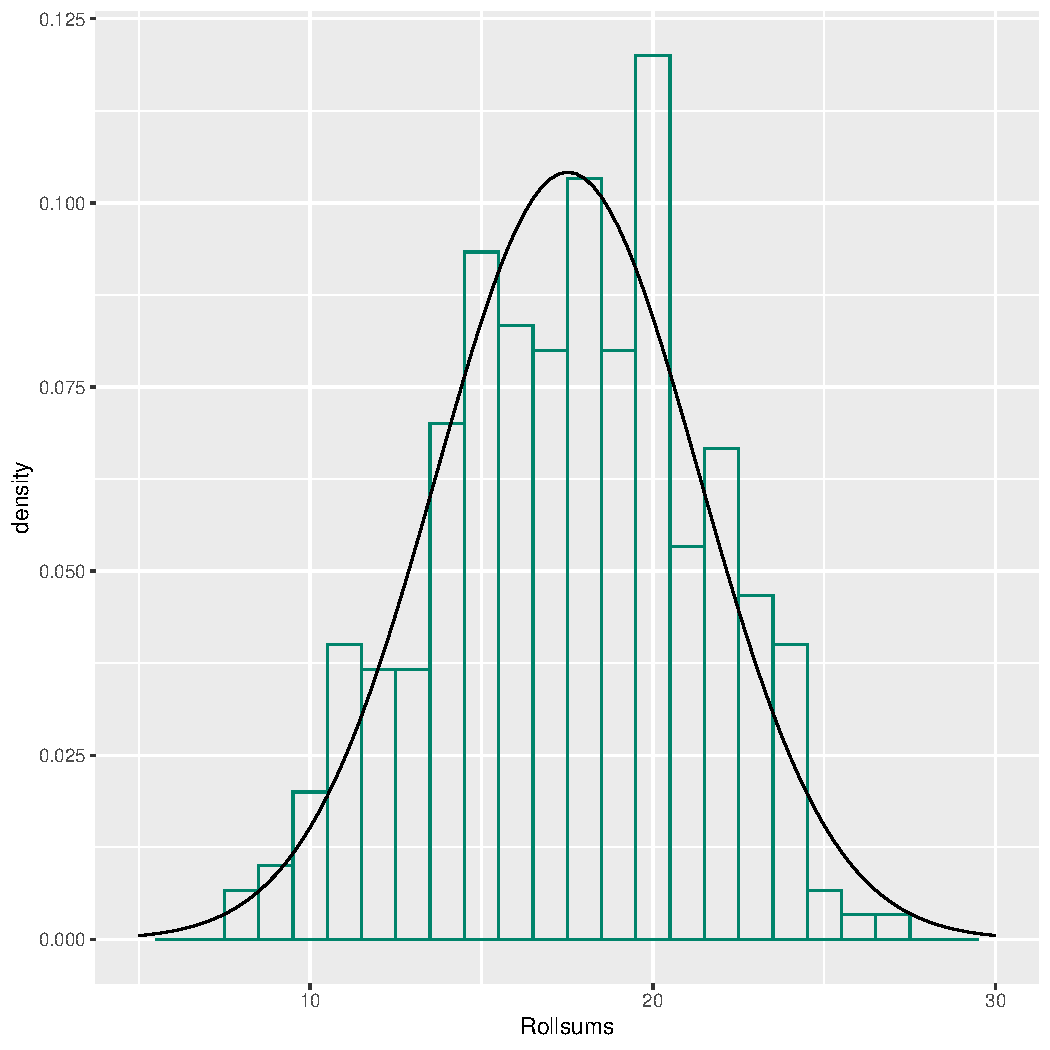
\includegraphics[width=\maxwidth]{figure/unnamed-chunk-11-1} 
\begin{kframe}\begin{alltt}
\hlcom{#and plots it with parameters a = mu and s = sigma, along x}
\end{alltt}
\end{kframe}
\end{knitrout}
    We simulate a bunch of trials where $5$ die are rolled and their respective rolls summed, We then take these sums and plot them in a proportion based histogram to which we fit the appropriate normal distribution's pdf which finally shows us that these sums approximately follow a normal distribution with mean being the average sum, which by linearity of expectation is approximately $5\times(1+2+3+4+5)/5=15$ and standard deviation being the standard deviation of these sums, which being roughly independendent makes this be approximately $\sqrt{5\times\text{the standard deviation for a single roll}}$ by linearity of variance. 
\end{enumerate}
\end{document}
